\documentclass[10pt]{beamer}
\usetheme{Madrid}
\usepackage[T1]{fontenc}
\usepackage[utf8]{inputenc}
\usepackage[brazil]{babel}
\usepackage{lmodern}
\usepackage{hyperref}
\usepackage{listings}
\usepackage{xcolor}
\setbeamertemplate{navigation symbols}{}

\lstset{
  language=C++,
  basicstyle=\ttfamily\small,
  keywordstyle=\color{blue},
  commentstyle=\color{gray},
  stringstyle=\color{red},
  breaklines=true,
  showstringspaces=false,
}

\title{I/O Digital e Analógica}
\subtitle{Curso de Microcontroladores}
\author{}
\date{}

\begin{document}

\begin{frame}
  \titlepage
\end{frame}

\begin{frame}{Digital vs Analógico}
  \begin{itemize}
    \item Sinal digital é só 0 ou 1, `LOW` (0V) ou `HIGH` (5V).
    \item Sinal analógico varia continuamente em um intervalo.
    \item Para ler dados analógicos, usamos `analogRead()`, que retorna um valor entre 0-1023.
    \item Não existem valores analógicos no mundo digital (Microcontroladores), então trabalhamos com ADCs (Analog to Digital Converters) para ler sinais analógicos.
    \item Para dados de saída, o `analogWrite()` simula analógico usando PWM (Pulse Width Modulation).
  \end{itemize}
\end{frame}

\begin{frame}{Conversão analógica-digital}
  \begin{itemize}
    \item Sensores analógicos leem a intensidade luminosa da pista (QTR, LDR, IR).
    \item Convertem isso a valores 0-1023 (varia, pode ir até 2055 ou 4095).
    \item Essa conversão é feita pelo ADC interno do microcontrolador, seguindo os passos de amostragem, quantização e codificação.
    \begin{figure}
      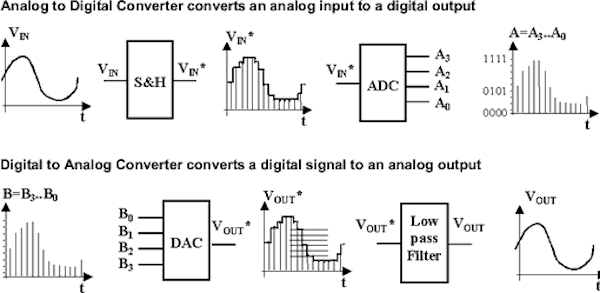
\includegraphics[width=0.8\textwidth]{adc.png}
      \caption{Processo de conversão analógico-digital}
    \end{figure}
  \end{itemize}
\end{frame}

\begin{frame}{Como funciona o PWM?}
  \begin{itemize}
    \item No PWM, uma onda retangular varia a largura do seu pulso, e essa variação controla o quanto uma segunda onda vai crescer ou diminuir.
    \begin{figure}
      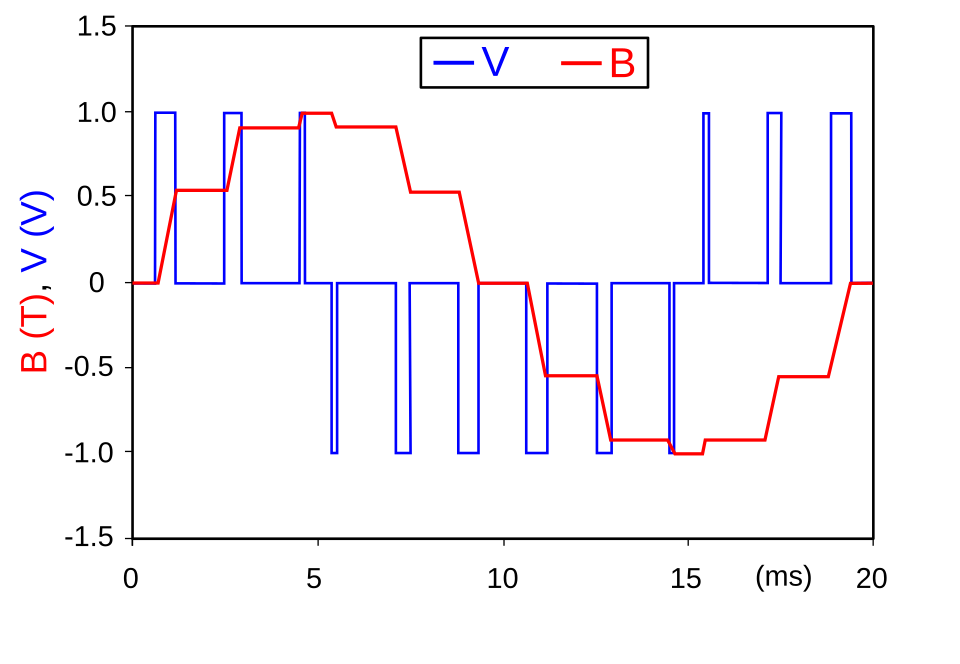
\includegraphics[width=0.8\textwidth]{pwm.png}
      \caption{Exemplo de PWM}
    \end{figure}
    % Many digital circuits can generate PWM signals (e.g., many microcontrollers have PWM outputs). They normally use a counter that increments periodically (it is connected directly or indirectly to the clock of the circuit) and is reset at the end of every period of the PWM. When the counter value is more than the reference value, the PWM output changes state from high to low (or low to high).[7] This technique is referred to as time proportioning, particularly as time-proportioning control[8] – which proportion of a fixed cycle time is spent in the high state.

    \item O ciclo de trabalho (duty cycle) é a porcentagem do tempo que o sinal fica `HIGH` em um período.
    \item No caso dos microcontroladores, existe um contador que incrementa periodicamente e é resetado no final de cada período do PWM. Quando o valor do contador é maior que um valor de referência, a saída do PWM muda de estado (de `HIGH` para `LOW` ou vice-versa).
    \item O ciclo de trabalho pode ser variado em passos discretos, dependendo da resolução do contador.
  \end{itemize}
\end{frame} 

\begin{frame}{Por que é importante entender o PWM para microcontroladores?}
  \begin{itemize}
    \item Quando usamos o PWM no `analogWrite()`, o sinal na verdade é digital, porém, simula-se um sinal analógico.
    \item Mas como entender PWM afeta no uso do `analogWrite()`, se ele mesmo já faz isso para mim?
    \item O `analogWrite()` é uma função de alto nível que abstrai o controle do PWM, mas entender o que acontece por baixo dos panos é fundamental.
    \item Por exemplo, se eu tiver um problema envolvendo o motor, saber que o PWM é uma onda retangular me ajuda a diagnosticar se o problema é no sinal de controle ou no motor em si.

  \end{itemize}
\end{frame}

\begin{frame}{Por que é importante entender o PWM para microcontroladores?}
  \begin{itemize}
    \item Mas se a saída é PWM, como ocorre essa transformação para o sinal semi-analógico que o motor recebe? 
    \item Quando o PWM envia um pulso HIGH, a corrente sobe gradualmente. Quando o sinal vai para LOW, a energia armazenada no campo magnético da bobina faz a corrente continuar fluindo por um breve momento.
    \item Isso transforma a onda quadrada de tensão em uma onda triangular de vários 'degraus'
    \item Ou seja, o sinal não sai pronto do microcontrolador. A menos que o equipamento tenha algo que transforme a onda PWM em analógica (bobinas, circuito buck), será necessário montar um circuito para isso
    \item Curiosamente, LEDs funcionam com PWM por um efeito chamado dimerização
    
  \end{itemize}
\end{frame}

\begin{frame}[fragile]{Leitura analógica e PWM}
\begin{lstlisting}
const int POT_PIN = A0;
const int LED_PIN = 9;

void loop() {
  int valorPot = analogRead(POT_PIN);
  int intensidade = map(valorPot, 0, 1023,
                        0, 255);
  analogWrite(LED_PIN, intensidade);
}
\end{lstlisting}

  \begin{itemize}
    \item `map()` converte de um intervalo para outro.
    \item `analogWrite()` funciona em pinos com PWM (~3, ~5, ~6, ~9, ~10, ~11).
    \item Não são todos os pintos de um microcontrolador que suportam PWM, então é importante verificar a documentação.
  \end{itemize}
\end{frame}

\begin{frame}[fragile]{Exemplo completo}
\begin{lstlisting}
const int BUTTON_PIN = 2;
const int POT_PIN = A0;
const int LED_PIN = 9;

void setup() {
  pinMode(BUTTON_PIN, INPUT_PULLUP);
  pinMode(LED_PIN, OUTPUT);
}

void loop() {
  int estadoBotao = digitalRead(BUTTON_PIN);
  int valorPot = analogRead(POT_PIN);
  int intensidade = map(valorPot, 0, 1023,
                        0, 255);
  if (estadoBotao == LOW) {
    analogWrite(LED_PIN, intensidade);
  } else {
    analogWrite(LED_PIN, 0);
  }
  delay(50);
}
\end{lstlisting}
\end{frame}


\begin{frame}{PWM no ESP32}
  \begin{itemize}
    \item ESP32 tem mais flexibilidade com PWM que Arduino tradicional.
    \item Muitos pinos podem gerar PWM simultaneamente.
    \item Usa canais independentes (16 canais disponíveis).
    \item Cada canal tem frequência, resolução e duty cycle próprios.
    \item Para configurar, usamos `ledcAttach()` para associar um pino a um canal PWM.
    \item O uso de frequências diferentes é útil para controlar dispositivos que exigem diferentes características de sinal (ex: motores vs LEDs).
    \item A resolução afeta o quão definido o controle vai ser, ou seja, quanto maior a resolução, mais definido será o sinal.
  \end{itemize}
\end{frame}

\begin{frame}[fragile]{Introdução a `ledcAttach()` no ESP32}
\begin{lstlisting}
// ledcAttach(pino, frequencia, resolucao)
ledcAttach(pino_motor, 5000, 8);

// Depois controlar com ledcWrite()
ledcWrite(pino_motor, 200);  // valor 0-255
\end{lstlisting}

  \begin{itemize}
    \item `pino`: o pino GPIO a usar.
    \item `frequencia`: em Hz (5000 Hz é padrão para motores).
    \item `resolucao`: bits (8 bits = 0-255, 10 bits = 0-1023).
  \end{itemize}
\end{frame}

\begin{frame}{Entendendo os argumentos de `ledcAttach()`}
  \begin{itemize}
    \item \textbf{Frequência}: quanto mais alta, menos ruído (mas mais consumo).
    \item Frequência >10kHz: imperceptível, ótimo para motores.
    \item Frequência <10Hz: visível a olho nu (LED piscando).
    \item \textbf{Resolução}: quantos bits para precisão do duty cycle.
    \item 8 bits (0-255): adequado para a maioria dos motores.
    \item 10 bits (0-1023): controle mais fino se necessário.
  \end{itemize}
\end{frame}

\begin{frame}[fragile]{`ledcAttach()` vs `ledcAttachPin()` (antigo)}
\begin{lstlisting}
// ANTIGO (ainda funciona, mas deprecado)
ledcSetup(canal, frequencia, resolucao);
ledcAttachPin(pino, canal);  // manual

// NOVO (ESP-IDF v5.0+)
ledcAttach(pino, frequencia, resolucao);
\end{lstlisting}

  \begin{itemize}
    \item `ledcAttachPin()`: requer gerenciar canal manualmente.
    \item `ledcAttach()`: aloca canal automaticamente (simpler!).
    \item `ledcAttach()` retorna o canal alocado.
    \item Preferir `ledcAttach()` em código novo.
  \end{itemize}
\end{frame}

\begin{frame}[fragile]{Exemplo com múltiplos motores}
\begin{lstlisting}
const int MOTOR_ESQ = 25;
const int MOTOR_DIR = 26;

void setup() {
  ledcAttach(MOTOR_ESQ, 5000, 8);
  ledcAttach(MOTOR_DIR, 5000, 8);
}

void loop() {
  ledcWrite(MOTOR_ESQ, 150);  // 59%
  ledcWrite(MOTOR_DIR, 200);  // 78%
  delay(1000);
  ledcWrite(MOTOR_ESQ, 0);
  ledcWrite(MOTOR_DIR, 0);
}
\end{lstlisting}
\end{frame}

\begin{frame}{Aplicação no seguidor de linha}
  \begin{itemize}
    \item Use `ledcAttach()` para cada motor.
    \item Frequência 5000 Hz é padrão para motores DC.
    \item Resolução 8 bits é suficiente para controle de velocidade.
    \item `ledcWrite()` muda velocidade em tempo real.
    \item PID ajusta valores de `ledcWrite()` continuamente.
    \item Cada canal é independente, pode ter configurações diferentes.
  \end{itemize}
\end{frame}

\end{document}
